\documentclass{article}

\ttfamily

\usepackage{graphicx}       % Loads images
\usepackage{subfig}
\graphicspath{{images/}}    % Set the default location for images

\usepackage{hyperref}
\hypersetup{pdftitle={Play Dead user manual}}

\begin{document}
 \title{Play Dead}
 \author{Fahmi Abdulhamid, Dan Cope, Daniel Atkins,\\Tim Jones, Carson Bruce, Liam Cervante}
 \date{June 2012}
 \maketitle
 
 \section{About}Play Dead was created for the National Game Development Month. We are 6 students at Victoria University of Wellington and we hope you enjoy our game.
 \begin{itemize}
  \item Links:
  \begin{itemize}
   \item \url{http://www.nagademo.com}
   \item \url{https://github.com/zimothy/play-dead}
  \end{itemize}
 \end{itemize}
 
 \section{Introduction}
 
 You are John \emph{``Danger''} Smith. You have awoken in a dark castle with no recollection as to how you got here. You can feel someone watching you, some dark presence with bad intentions. You feel yourself getting sleepy as footsteps approach.
 
 You awaken again to find yourself in a room with nothing except a ladder and a switch and no visible exit. What awaits is a terrifying journey that will damage your very soul.
 
 \section{Controls}
 
 WASD or arrow keys control your movement and E activates switches. The challenge is now making your way through the castle and, hopefully, eventual escape.
 
 \section{Ending}
 
 As you make your way through the castle solving problems, going from room to room, you realise you have no way of escaping. Maybe, if you continue on the dark journey the presence will take pity on you and let you leave.
 
 \section{Game Objects}

\begin{figure}[htb]
    \centering
    \subfloat[John \emph{``Danger''} Smith (that's you).]
    {
        
\includegraphics[width=0.28\linewidth]{player}
    }
    \hfill
    \subfloat[Spawner. When you die, you are cloned here.]
    {
        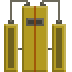
\includegraphics[width=0.28\linewidth]{spawner}
    }
    \hfill
    \subfloat[Exit. Escape the level.]
    {
        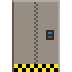
\includegraphics[width=0.28\linewidth]{exit}
    }
    
    \subfloat[Switch. Use to active doors and spawners.]
    {
        
\includegraphics[width=0.28\linewidth]{switch}
    }
    \hfill
    \subfloat[Wheel. Crank to pump water from one space to another.]
    {
        
\includegraphics[width=0.28\linewidth]{wheel}
    }
    \hfill
    \subfloat[Laser. Connect lasers to make a circuit.]
    {
        
\includegraphics[width=0.28\linewidth]{laser}
    }

    \subfloat[Spikes. Don't touch them!]
    {
        
\includegraphics[width=0.28\linewidth]{spikes}
    }
    \hfill
    \subfloat[Water. You can't swim...]
    {
        
\includegraphics[width=0.28\linewidth]{water}
    }
    \hfill
    \subfloat[Ladder. For climbing.]
    {
        
\includegraphics[width=0.28\linewidth]{ladder}
    }
    \caption{iRemember interface screenshots.}
    \label{fig_iRemember}
\end{figure}
 
 \section{Special thanks}
 We would acknowledge the use of the following work:
 
\begin{itemize}
	\item Microsoft XNA Platformer Starter Kit: \url{http://msdn.microsoft.com/en-us/library/dd254918\%28v=xnagamestudio.31\%29.aspx}
	\item Mechanical2.wav by BMacZero: \url{http://www.freesound.org/people/BMacZero/sounds/94121/}
	\item Clank1.wav by BMacZero: \url{http://www.freesound.org/people/BMacZero/sounds/94127/}
	\item horror ambience 12.wav by klankbeeld: \url{http://www.freesound.org/people/klankbeeld/sounds/133659/}
\end{itemize}
 
\end{document}
